\subsubsection{28.11.2015}
\textit{\textbf{Time frame:}} 17:00-21:30 \newline
Blocks were installed onto the angles on the elevator.
The concept of the winch was changed. It was decided to apply 3 standard DC motors with gear ratio 1:1. 3 standard TETRIX motors with torque 10 kg/cm and speed 2 r/pm are able to pull up robot of 10 kg with a speed $3 \cdot 2\pi \cdot 2 = 38$ cm/s. Incliding safety coefficient 1.5 the speed will amount to 25 cm/s. Since the overal length of the cable required for pulling up from 1-st zone is about 1m, the robot will be able to pull up in 4 seconds. The time of the full extracting of the elevator would be the same.

\begin{figure}[H]
	\begin{minipage}[h]{0.47\linewidth}
		\center{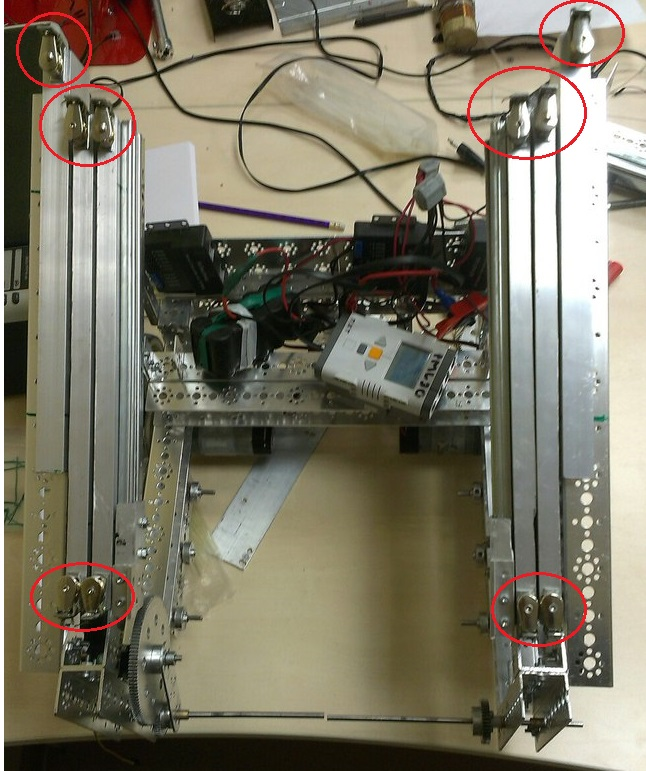
\includegraphics[scale=0.25]{3Engineering/5Team_meetings/days_of_meetings/2015.11.28/images/01}}
		\caption{Blocks on the elevator}
	\end{minipage}
	\hfill
	\begin{minipage}[h]{0.47\linewidth}
		\center{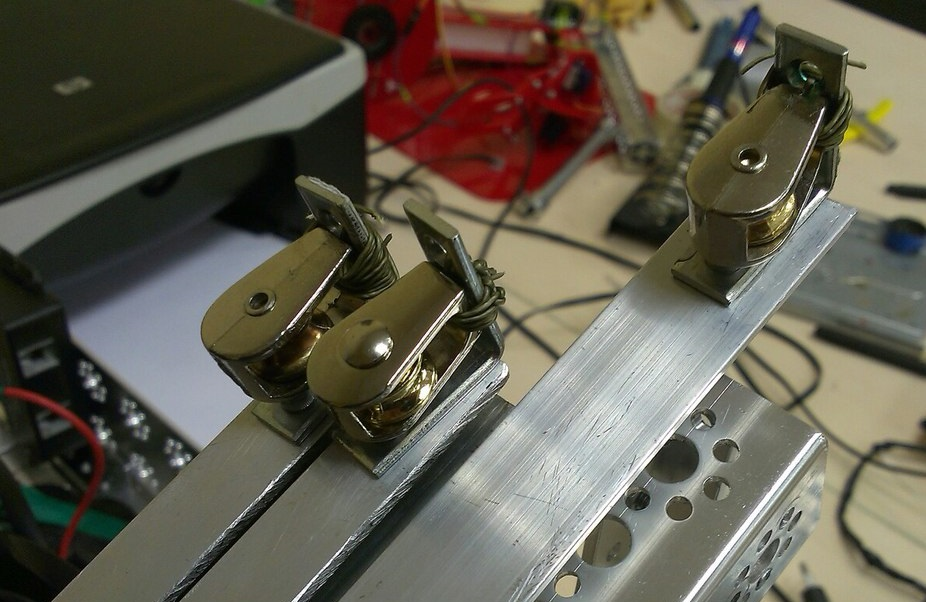
\includegraphics[scale=0.25]{3Engineering/5Team_meetings/days_of_meetings/2015.11.28/images/02}}
		\caption{Blocks}
	\end{minipage}
\end{figure} 